\documentclass[pdftex,a4paper,12pt,abstracton]{scrartcl}

\usepackage[latin9]{inputenc}
\usepackage[T1]{fontenc}
\usepackage{xcolor}
\usepackage{graphicx}
\usepackage{amsmath, amsthm, amssymb}
%\usepackage{ngerman}
%\usepackage{bibgerm}
%\usepackage[ngerman]{translator}
\usepackage{longtable}
\usepackage{listings}
\usepackage{float}
\usepackage{color}
\usepackage{geometry}
\geometry{left=3cm, textwidth=16cm, top=3cm, textheight=24cm}
\usepackage{relsize}
\usepackage[round, sort]{natbib}
\usepackage{indentfirst}
\usepackage{scrpage2}
\usepackage{soul}
\usepackage{listings}
\pagestyle{scrheadings}
\definecolor{red}{rgb}{1,0,0}
\setstcolor{red}


 
%\renewcommand*{\chapterpagestyle}{scrheadings}
\clearscrheadfoot
\ihead{\headmark}
\ohead{\pagemark}
\setheadsepline{.4pt}
\newcommand*{\xchapter}{\setcounter{chapter}{0}\addchap}

\newcommand{\dd}{\mathrm{d}} 

\newcommand\note[1]{\textcolor{red}{#1}}
\newcommand\noteit[1]{\textcolor{red}{\textit{#1}}}

\title{The GalerkinTools library: Efficient implementation of Galerkin type finite element formulations}
\author{\large Sebastian Stark$^1$}
\date{\footnotesize \textit{$^1$Centre for Research in Computational and Applied Mechanics, University of Cape Town, 7701 Rondebosch, South Africa}}

%\renewcommand{\baselinestretch}{1.5}

\begin{document}

\maketitle

\section{Introduction}
The numerical solution of problems from continuum mechanics and related fields by means of Galerkin type finite element methods usually follows the same general steps. Despite this fact, most commercial finite element codes are limited to certain standard applications. In the case of non-standard applications on the contrary, it is necessary to develop custom codes. In this context, open source finite element libraries like deal.II \citep{bangerth2007, alzetta2018} provide a powerful framework comprising implementations of the standard building blocks of finite element software. Still, a significant amount of coding is often necessary to implement a numerical scheme for a particular problem. This applies especially to the assembly of the finite element system. Although, for most problems, the really problem specific part boils down to a few simple functions emerging already in the continuous setting (and certain derivatives thereof), the implementation of the assembly procedures is usually a tedious and error prone task. This has motivated the development of the GalerkinTools library, which is based on deal.II and assists the user during assembly for the case that the finite element formulation is obtained based on a standard Galerkin approach. In particular, the task of the user is essentially reduced to the definition of the underlying weak form in a suitable way, the finite element mesh, the finite element space, and, possibly, constraints applying to the latter. The main purpose of this note is to describe (i) the problem type which can be handled by the GalerkinTools library, (ii) the main steps necessary to define the problem in practice, and (iii) some of the internal procedures of the GalerkinTools library.

\section{Spatially continuous problem under consideration}
In the following, the weak form under consideration is described. In this context, it is for formal reasons pretended that a scalar valued potential function $\Pi$ exists such that the weak form follows from the requirement that the first variation of $\Pi$ vanishes. However, the problems which can be handled by the GalerkinTools library need not necessarily be associated with such a potential.

It is also remarked that no explicit dependence on time is considered. However, time dependent problems can still be handled if the weak form is already discrete in time.

\subsection{Spatial domain and interfaces}
\begin{figure}[htb]
\centering
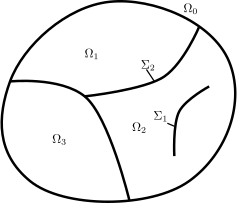
\includegraphics[scale=1.0]{graphics/domain.pdf}
\caption{Domain under consideration.}
\label{domain}
\end{figure}
The Euclidean $n$-space $\mathbb{R}^n$ with $n=2$ or $n=3$ is considered. $\mathbb{R}^n$ is split into the ``computational domain'' $\Omega \subset \mathbb{R}^n$ and the ``environment'' $\Omega_0 = \mathbb{R}^n \setminus \Omega$, see also Figure \ref{domain}. The computational domain is further subdivided into ``domain portions'' $\Omega_\alpha$, where $\alpha \in A=\left\{1, \hdots, N^\mathrm{\Omega}\right\}$, $\bigcup_{\alpha \in A} \Omega_\alpha = \Omega$, and $\Omega_\alpha \cap \Omega_\beta = 0$ if $\alpha\neq \beta$. Additionally, the $n-1$ dimensional ``interface'' $\Sigma$ is introduced. This interface is further subdivided into ``interface portions'' $\Sigma_\gamma$, where $\gamma \in \Gamma=\left\{1, \hdots, N^\mathrm{\Sigma}\right\}$, and $\Sigma_\gamma \cap \Sigma_\delta = 0$ if $\gamma\neq \delta$. Interface portions may align with interfaces between the domain portions $\Omega_\alpha$ or the interface between $\Omega$ and $\Omega_0$, but need not to. Together with the interface, a piecewise continuous unit normal field $\boldsymbol{n}(\boldsymbol{X})$ satisfying $\boldsymbol{n}(\boldsymbol{X})\cdot\boldsymbol{n}(\boldsymbol{X}) = 1$ is defined. Using this normal field, the '$+$' and '$-$' sides of the interface at a point $\boldsymbol{X} \in \Sigma$ are defined such that $\boldsymbol{n}(\boldsymbol{X})$ points from $-$ to $+$.

\subsection{Unknowns of the problem: independent fields and scalars}
The unknowns of the problem are a set of ``independent fields'' and, possibly, a set of ``independent scalars''. The independent fields may either be related to the domain (or portions thereof) or to the interface (or portions thereof), while the independent scalars have no spatial association.

The ``domain related independent fields'' $u^\Omega_\epsilon \in \mathcal{V}^\Omega_\epsilon \subseteq \mathcal{L}^2(\mathbb{R}^n)$ are introduced according to\footnote{Defining $u^\Omega_\epsilon$ on the entire $\mathbb{R}^n$ instead of on  $\Omega$ has the advantage that the boundary of the domain can formally be considered as an interface. The latter viewpoint is also physically motivated: A boundary may be seen as a special interface, where the situation on one side of it is known to some extent (in particular, to the extent it influences the situation on the other side of the boundary).}
\begin{equation}
u^\Omega_\epsilon:
\begin{cases}
\mathbb{R}^n \rightarrow \mathbb{R}\\
\boldsymbol{X} \mapsto u^\Omega_\epsilon(\boldsymbol{X}),
\end{cases}
\end{equation}
where $\epsilon \in E=\left\{1, \hdots, N^\mathrm{u,\Omega}\right\}$, and $\boldsymbol{X}\in \mathbb{R}^n$.

Similarly, the ``interface related independent fields'' $u^\Sigma_\eta \in \mathcal{V}^\Sigma_\eta \subseteq \mathcal{L}^2(\Sigma)$ are introduced according to
\begin{equation}
u^\Sigma_\eta:
\begin{cases}
\Sigma \rightarrow \mathbb{R}\\
\boldsymbol{X} \mapsto u^\mathrm{\Sigma}_\eta(\boldsymbol{X}),
\end{cases}
\end{equation}
where $\eta \in H=\left\{1, \hdots, N^\mathrm{u,\Sigma}\right\}$.

It will generally be assumed that $u^\Omega_\epsilon(\boldsymbol{X}) = 0$ if $\boldsymbol{X} \in \Omega_0$. Also, sets $A_{\epsilon,u\neq 0} \subset A$ and $\Gamma_{\eta,u\neq 0} \subset \Gamma$ are introduced. If $\alpha \notin A_{\epsilon,u\neq 0}$, then $u^\Omega_\epsilon(\boldsymbol{X})=0$ if $\boldsymbol{X} \in \Omega_\alpha$. Similarly, if
$\gamma \notin \Gamma_{\eta,u\neq 0}$, then $u^\Sigma_\eta(\boldsymbol{X})=0$ if $\boldsymbol{X} \in \Sigma_\gamma$. I.e., the sets $A_{\epsilon,u\neq 0}$ and $\Gamma_{\eta,u\neq 0}$ determine on which domain portions and interface portions the unknown fields $u^\Omega_\epsilon$ and $u^\Sigma_\eta$ may be non-zero, and on which domain and interface portions they are constrained to zero. This approach effectively allows for different sets of unknown fields on different domain/interface portions. In addition, further problem specific constraints may apply to $u^\Omega_\epsilon$ and $u^\Sigma_\eta$. It is understood that all constraints as well as regularity requirements on the independent fields are incorporated by choosing appropriate spaces $\mathcal{V}^\Omega_\epsilon$ and $\mathcal{V}^\Sigma_\eta$. Moreover, it is noted that, although each independent field is scalar valued, tensor valued unknown fields can easily be accounted for by combining several scalar valued fields.

Finally, the ``independent scalars'' $C_\iota \in \mathbb{R}$ are introduced, where $\iota \in I=\left\{1, \hdots, N^\mathrm{C}\right\}$. Hence, the unknowns of the problem are $(u^\Omega_\epsilon, u^\Sigma_\eta, C_\iota)$.

\subsection{Dependent fields}
The ``domain related dependent fields'' are introduced according to
\begin{equation}
e^\Omega_\lambda = \sum_{\epsilon \in E} \left[ a^\Omega_{\lambda\epsilon} u^\Omega_\epsilon + \boldsymbol{b}^\Omega_{\lambda \epsilon} \cdot (\nabla u^\Omega_\epsilon) \right] + \sum_{\iota \in I}c^\Omega_{\lambda\iota} C_\iota  + d^\Omega_\lambda.
\label{dependent_field_domain}
\end{equation}
Here, $\lambda \in \Lambda=\left\{1, \hdots, N^{\mathrm{e},\Omega}\right\}$; $a^\Omega_{\lambda\epsilon}$, $c^\Omega_{\lambda\iota}$ and $d^\Omega_\lambda$ are constants; and $\boldsymbol{b}^\Omega_{\lambda\epsilon}$ are constant vectors.

Similarly, the ``interface related dependent fields'' are introduced according to
\begin{equation}
\begin{split}
e^\Sigma_\nu &=  \sum_{\eta \in H} \left[ a^\Sigma_{\nu\eta} u^\Sigma_\eta + \boldsymbol{b}^\Sigma_{\nu\eta} \cdot (\nabla u^\Sigma_\eta) \right]\\
             & + \sum_{\epsilon \in E} \left[ a^+_{\nu\epsilon} (u^\Omega_\epsilon)^+ + \boldsymbol{b}^+_{\nu\epsilon} \cdot (\nabla u^\Omega_\epsilon)^+ \right]\\
             & + \sum_{\epsilon \in E} \left[ a^-_{\nu\epsilon} (u^\Omega_\epsilon)^- + \boldsymbol{b}^-_{\nu\epsilon} \cdot (\nabla u^\Omega_\epsilon)^- \right]\\
             & + \sum_{\iota \in I}c^\Sigma_{\nu\iota} C_\iota + d^\Sigma_\nu.
\end{split}
\label{dependent_field_interface}
\end{equation}
Here, $\nu \in N=\left\{1, \hdots, N^\mathrm{e,\Sigma}\right\}$; and $a^\Sigma_{\nu\eta}$, $a^+_{\nu\epsilon}$, $a^-_{\nu\epsilon}$,  $c^\Sigma_{\nu\iota}$ and $d^\Sigma_\nu$ are constants; and $\boldsymbol{b}^\Sigma_{\nu\eta}$, $\boldsymbol{b}^+_{\nu\epsilon}$, $\boldsymbol{b}^-_{\nu\epsilon}$ are constant vectors. The superscript $+/-$ on a domain related independent field indicates that it is evaluated on the $+/-$ side of the interface.

The concept of dependent fields is used to define quantities which are derived from the set of unknowns in terms of linear relations. For illustration of the concept, consider an electrostatics problem with the scalar potential $\varphi$ as an independent field defined on the domain. Then, dependent fields would be the electric field components, which are the components of the negative of the gradient of $\varphi$. It is also remarked that the trivial case that a dependent field equals an independent field  is explicitly allowed for.

\subsection{Scalar functionals}
A set of scalar valued ``domain related scalar functionals'' is introduced according to
\begin{equation}
H^\Omega_\rho = \int_\Omega h^\Omega_\rho(e^\Omega_\lambda, \boldsymbol{X}) \mathrm{d}V,
\end{equation}
where $\rho \in P=\left\{1, \hdots, N^\mathrm{H,\Omega}\right\}$, and the $h^\Omega_\rho$ are problem specific functions, which may be nonlinear.

Similarly, a set of scalar valued ``interface related scalar functionals'' is introduced according to
\begin{equation}
H^\Sigma_\tau = \int_\Sigma h^\Sigma_\tau(e^\Sigma_\nu, \boldsymbol{X}) \mathrm{d}S,
\end{equation}
where $\tau \in T=\left\{1, \hdots, N^\mathrm{H,\Sigma}\right\}$, and the $h^\Sigma_\tau$ are again problem specific functions, which may be nonlinear.

In the same way as for the independent fields, sets $A_{\rho,h\neq 0} \subset A$ and $\Gamma_{\tau,h\neq 0} \subset \Gamma$ are introduced. If $\alpha \notin A_{\rho,h\neq 0}$, then $h^\Omega_\rho(e^\Omega_\lambda, \boldsymbol{X})=0$ if $\boldsymbol{X} \in \Omega_\alpha$. Similarly, if
$\gamma \notin \Gamma_{\tau,h\neq  0}$, then $h^\Sigma_\tau(e^\Sigma_\nu, \boldsymbol{X})=0$ if $\boldsymbol{X} \in \Sigma_\gamma$. I.e., the sets $A_{\epsilon,h\neq 0}$ and $\Gamma_{\eta,h\neq 0}$ determine on which domain portions and interface portions the functions $h^\Omega_\rho$ and $h^\Sigma_\tau$ may be non-zero, and on which domain and interface portions they are set to zero. This approach effectively allows for different sets of scalar functionals on different domain/interface portions.

\subsection{Scalar valued potential and weak form}
Based on the previously introduced quantities, the scalar valued potential is finally written as
\begin{equation}
\Pi=\Pi(H^\Omega_\rho, H^\Sigma_\tau, C_\iota);
\label{Pi}
\end{equation}
and the equations determining the unknown fields are obtained by requiring that the first variation of $\Pi$ be stationary.

Using the definitions
\begin{equation}
\begin{split}
\Pi^\Omega_\rho      &= \dfrac{\partial \Pi}{\partial H^\Omega_\rho},\\
\Pi^\Sigma_\tau      &= \dfrac{\partial \Pi}{\partial H^\Sigma_\tau},\\
\Pi^\mathrm{C}_\iota &= \dfrac{\partial \Pi}{\partial C_\iota},\\
h^\Omega_{\rho \lambda}     &= \dfrac{\partial h^\Omega_\rho}{\partial e^\Omega_\lambda},\\
h^\Sigma_{\tau \nu}  &= \dfrac{\partial h^\Sigma_\tau}{\partial e^\Sigma_\nu}
\end{split}
\end{equation}
and the usual notation of variational calculus, the condition for $\Pi$ to be stationary may be expressed as
\begin{multline}
  \delta \Pi(u^\Omega_\epsilon, u^\Sigma_\eta, C_m, \delta u^\Omega_\epsilon, \delta u^\Sigma_\eta, \delta C_\iota)
  =
    \sum_{\rho \in P} \sum_{\lambda \in \Lambda} \Pi^\Omega_\rho \int_\Omega h^\Omega_{\rho \lambda} \delta e^\Omega_\lambda \mathrm{d}V
  + \sum_{\tau \in T} \sum_{\nu \in N} \Pi^\Sigma_\tau \int_\Sigma h^\Sigma_{\tau\nu} \delta e^\Sigma_\nu \mathrm{d}S\\
  + \sum_{\iota \in I} \Pi^\mathrm{C}_\iota \delta C_\iota
  = 0
  \quad \forall (\delta u^\Omega_\epsilon, \delta u^\Sigma_\eta, \delta C_\iota).
  \label{stationarity_conditions}
\end{multline}
The latter weak form defines the problem under consideration. In the following, it will be assumed that this problem is well-posed.

\subsection{Remarks}
\label{remarks}
\begin{enumerate}
\item As indicated earlier, Eq.\@ \eqref{stationarity_conditions} can still be used for the determination of the unknowns $(u^\Omega_\epsilon, u^\Sigma_\eta, C_\iota$) if $\Pi$ does not exist and only $\Pi^\Omega_\rho$, $\Pi^\Sigma_\tau$, and $\Pi^\mathrm{C}_\iota$ are defined. Furthermore, if $\Pi^\Omega_\rho$, $\Pi^\Sigma_\tau$, and $\Pi^\mathrm{C}_\iota$ are all independent of a particular $H^\Omega_\rho$ (or $H^\Sigma_\tau$), it is not necessary to give a relation for that $H^\Omega_\rho$ (or $H^\Sigma_\tau$). Rather, it is then sufficient, to define $h^\Omega_{\rho\lambda}$ (or $h^\Sigma_{\tau\nu}$). However, existence of $\Pi$ is a desirable property because (i) the mathematical analysis of the problem is typically simplified, and (ii) the resulting finite element system is usually symmetric.

\item A restriction of \eqref{stationarity_conditions} is that only up to first derivatives of the unknown fields are allowed for. Despite this limitation, problems involving higher derivatives may still be treated within the present framework by using auxiliary independent fields representing higher derivatives of the unknown fields and incorporating the resulting constraints by a Lagrangian multiplier approach. In the context of finite element analysis, this approach is often also advantageous because the requirement of higher order continuous finite elements is circumvented.

\item The introduction of the independent scalars $C_\iota$ together with the assumption of a general function for $\Pi$ (instead of just adding the scalar functions $H^\Omega_\rho$ and $H^\Sigma_\tau$ up to a scalar valued potential) allow for the incorporation of certain integral type equations. These do, e.g., emerge in an electrostatics problem if a total electrical charge is to be prescribed on an electrode.
\end{enumerate}

\section{Spatially discrete problem under consideration}
The spatially discrete problem is obtained based on the weak form \eqref{stationarity_conditions} by the Galerkin approach. I.e., the approximate solution is given by those $u^{\Omega,\mathrm{h}}_\epsilon \in \mathcal{V}^{\Omega,\mathrm{h}}_\epsilon$, $u^{\Sigma,\mathrm{h}}_\eta \in \mathcal{V}^{\Sigma,\mathrm{h}}_\eta$, $C^\mathrm{h}_\iota \in \mathbb{R}$ satisfying
\begin{equation}
  \delta \Pi(u^{\Omega,\mathrm{h}}_\epsilon, u^{\Sigma,\mathrm{h}}_\eta, C^\mathrm{h}_\iota, \delta u^{\Omega,\mathrm{h}}_\epsilon, \delta u^{\Sigma,\mathrm{h}}_\eta, \delta C^\mathrm{h}_\iota)
  = 0
  \quad \forall (\delta u^{\Omega,\mathrm{h}}_\epsilon, \delta u^{\Sigma,\mathrm{h}}_\eta, \delta C^\mathrm{h}_\iota),
  \label{stationarity_conditions_galerkin}
\end{equation}
where $\mathcal{V}^{\Omega,\mathrm{h}}_\epsilon \subset \mathcal{V}^\Omega_\epsilon$ and $\mathcal{V}^{\Sigma,\mathrm{h}}_\eta \subset \mathcal{V}^\Sigma_\eta$ are finite dimensional spaces.

Let $(w^{\Omega,\mathrm{h}}_{\epsilon \phi}, w^{\Sigma,\mathrm{h}}_{\eta \phi}, w^{\mathrm{C},\mathrm{h}}_{\iota \phi})$ with $\phi \in \Phi=\left\{1, \hdots, N^\mathrm{dof} \right\}$ be the $\phi$-th basis vector of a basis of the $N^\mathrm{dof}$-dimensional space $\mathcal{V}^{\Omega,\mathrm{h}}_0 \times \hdots \times \mathcal{V}^{\Omega,\mathrm{h}}_{N^\mathrm{u,\Omega}} \times \mathcal{V}^{\Sigma,\mathrm{h}}_0 \times \hdots \times \mathcal{V}^{\Sigma,\mathrm{h}}_{N^\mathrm{u,\Sigma}} \times \mathbb{R}^{N^\mathrm{C}}$.
Then, $u^{\Omega,\mathrm{h}}_\epsilon$, $u^{\Sigma,\mathrm{h}}_\eta$ and $C^\mathrm{h}_\iota$ may be expressed in terms of the scalar unknowns $\hat u_\phi$ according to
\begin{equation}
\begin{split}
u^{\Omega,\mathrm{h}}_\epsilon &= \sum_{\phi \in \Phi} \hat u_\phi w^{\Omega,\mathrm{h}}_{\epsilon\phi}\\
u^{\Sigma,\mathrm{h}}_\eta &= \sum_{\phi \in \Phi} \hat u_\phi w^{\Sigma,\mathrm{h}}_{\eta\phi}\\
C^\mathrm{h}_\iota &= \sum_{\phi \in \Phi} \hat u_\phi w^{\mathrm{C},\mathrm{h}}_{\iota\phi}.
\end{split}
\end{equation}
Also, it is readily seen that \eqref{stationarity_conditions_galerkin} is equivalent to require that
\begin{equation}
  \delta \Pi(u^{\Omega,\mathrm{h}}_\epsilon, u^{\Sigma,\mathrm{h}}_\eta, C^\mathrm{h}_\iota, w^{\Omega,\mathrm{h}}_{\epsilon\phi}, w^{\Sigma,\mathrm{h}}_{\eta\phi}, w^{\mathrm{C},\mathrm{h}}_{\iota\phi})
  = 0
  \quad \forall \phi \in \Phi,
  \label{stationarity_conditions_discrete}
\end{equation}
which are $N^\mathrm{dof}$ equations for the determination of the $N^\mathrm{dof}$ unknowns $\hat u_\phi$.

Assuming that the spatial discretization is based on the finite element method, the structure of the resulting finite element system will be discussed in the following. For this purpose, first the quantities
\begin{equation}
\begin{split}
h^\Omega_{\rho \lambda \mu} &= \dfrac{\partial h^\Omega_{\rho \lambda}}{\partial e^\Omega_\mu},\\
h^\Sigma_{\tau \nu \xi} &= \dfrac{\partial h^\Sigma_{\tau \nu}}{\partial e^\Sigma_\xi},\\
\Pi^{\Omega\Omega}_{\rho\sigma} &= \dfrac{\partial \Pi^{\Omega}_\rho}{\partial H^\Omega_\sigma},\quad
\Pi^{\Omega\Sigma}_{\rho\tau} = \dfrac{\partial \Pi^{\Omega}_\rho}{\partial H^\Sigma_\tau},\quad
\Pi^{\Omega\mathrm{C}}_{\rho\iota} = \dfrac{\partial \Pi^{\Omega}_\rho}{\partial C_\iota},\\
\Pi^{\Sigma\Omega}_{\tau\rho} &= \dfrac{\partial \Pi^{\Sigma}_\tau}{\partial H^\Omega_\rho},\quad
\Pi^{\Sigma\Sigma}_{\tau\upsilon} = \dfrac{\partial \Pi^{\Sigma}_\tau}{\partial H^\Sigma_\upsilon},\quad
\Pi^{\Sigma\mathrm{C}}_{\tau\iota} = \dfrac{\partial \Pi^{\Sigma}_\tau}{\partial C_\iota},\\
\Pi^{\mathrm{C}\Omega}_{\iota\rho} &= \dfrac{\partial \Pi^\mathrm{C}_\iota}{\partial H^\Omega_\rho},\quad
\Pi^{\mathrm{C}\Sigma}_{\iota\tau} = \dfrac{\partial \Pi^\mathrm{C}_\iota}{\partial H^\Sigma_\tau},\quad
\Pi^{\mathrm{C}\mathrm{C}}_{\iota\kappa} = \dfrac{\partial \Pi^\mathrm{C}_\iota}{\partial C_\kappa},\\
v^\Omega_{\lambda\phi} &= \sum_{\epsilon \in E} \left[ a^\Omega_{\lambda\epsilon} w^{\Omega,\mathrm{h}}_{\epsilon\phi} + \boldsymbol{b}^\Omega_{\lambda \epsilon} \cdot (\nabla w^{\Omega,\mathrm{h}}_{\epsilon\phi}) \right] + \sum_{\iota \in I}c^\Omega_{\lambda\iota} w^\mathrm{C,h}_{\iota\phi} ,\\
v^\Sigma_{\nu\phi} &=  \sum_{\eta \in H} \left[ a^\Sigma_{\nu\eta} w^{\Sigma,\mathrm{h}}_{\eta\phi} + \boldsymbol{b}^\Sigma_{\nu\eta} \cdot (\nabla w^{\Sigma,\mathrm{h}}_{\eta\phi}) \right]\\
                   & + \sum_{\epsilon \in E} \left[ a^+_{\nu\epsilon} (w^{\Omega,\mathrm{h}}_{\epsilon\phi})^+ + \boldsymbol{b}^+_{\nu\epsilon} \cdot (\nabla w^{\Omega,\mathrm{h}}_{\epsilon\phi})^+ \right]\\
                   & + \sum_{\epsilon \in E} \left[ a^-_{\nu\epsilon} (w^{\Omega,\mathrm{h}}_{\epsilon\phi})^- + \boldsymbol{b}^-_{\nu\epsilon} \cdot (\nabla w^{\Omega,\mathrm{h}}_{\epsilon\phi})^- \right]\\
                   & + \sum_{\iota \in I} c^\Sigma_{\nu\iota} w^\mathrm{C,h}_{\iota\phi},\\
v^\mathrm{C}_{\iota\phi} &= w^\mathrm{C,h}_{\iota\phi}
\end{split}
\end{equation}
are introduced. 
Furthermore, the vectors $\boldsymbol{f}^\Omega$, $\boldsymbol{f}^\Sigma$, $\boldsymbol{f}^\mathrm{C}$, and the matrices $\boldsymbol{K}^\Omega$, $\boldsymbol{K}^\Sigma$, $\boldsymbol{L}^\Omega$, $\boldsymbol{L}^\Sigma$ and $\boldsymbol{L}^\mathrm{C}$ are defined by
\begin{equation}
\begin{split}
f^\Omega_\phi &= \sum_{\rho \in P} \sum_{\lambda \in \Lambda} \Pi^\Omega_\rho \int_\Omega h^\Omega_{\rho\lambda} v^\Omega_{\lambda\phi} \mathrm{d}V,\\
f^\Sigma_\phi &= \sum_{\tau \in T} \sum_{\nu \in N} \Pi^\Sigma_\tau \int_\Sigma h^\Sigma_{\tau\nu} v^\Sigma_{\nu\phi} \mathrm{d}S,\\
f^\mathrm{C}_\phi &= \sum_{\iota \in I} \Pi^\mathrm{C}_\iota v^\mathrm{C}_{\iota\phi},\\
K^\Omega_{\phi\chi} &= \sum_{\rho \in P} \sum_{\lambda \in \Lambda} \sum_{\mu \in \Lambda} \Pi^\Omega_\rho \int_\Omega h^\Omega_{\rho \lambda \mu} v^\Omega_{\lambda\phi} v^\Omega_{\mu\chi} \mathrm{d}V,\\
K^\Sigma_{\phi\chi} &= \sum_{\tau \in T} \sum_{\nu \in N} \sum_{\xi \in N} \Pi^\Sigma_\tau \int_\Sigma h^\Sigma_{\tau \nu \xi} v^\Sigma_{\nu\phi} v^\Sigma_{\xi\chi} \mathrm{d}S,\\
L^\Omega_{\phi\rho} &= \sum_{\lambda \in \Lambda} \int_\Omega h^\Omega_{\rho\lambda} v^\Omega_{\lambda\phi} \mathrm{d}V,\\
L^\Sigma_{\phi\tau} &= \sum_{\nu \in N} \int_\Sigma h^\Sigma_{\tau\nu} v^\Sigma_{\nu\phi} \mathrm{d}S,\\
L^\mathrm{C}_{\phi\iota} &= v^\mathrm{C}_{\iota\phi}.
\end{split}
\end{equation}
Using these definitions, linearization of \eqref{stationarity_conditions_discrete} at a point $\boldsymbol{\hat u}$ yields the linear system
\begin{equation}
\underbrace{\boldsymbol{f}^\Omega + \boldsymbol{f}^\Sigma + \boldsymbol{f}^\mathrm{C}}_{\mbox{$\boldsymbol{f}$}} +
\left[
 \underbrace{\boldsymbol{K}^\Omega+
 \boldsymbol{K}^\Sigma}_{\mbox{$\boldsymbol{K}$}}+
 \underbrace{\begin{pmatrix}
  \boldsymbol{L}^\Omega & \boldsymbol{L}^\Sigma & \boldsymbol{L}^\mathrm{C}
 \end{pmatrix}}_{\mbox{$\boldsymbol{L}$}}
 \underbrace{
 \begin{pmatrix}
  \boldsymbol{\Pi}^{\Omega\Omega} & \boldsymbol{\Pi}^{\Omega\Sigma} & \boldsymbol{\Pi}^{\Omega\mathrm{C}} \\
  \boldsymbol{\Pi}^{\Sigma\Omega} & \boldsymbol{\Pi}^{\Sigma\Sigma} & \boldsymbol{\Pi}^{\Sigma\mathrm{C}} \\
  \boldsymbol{\Pi}^{\mathrm{C}\Omega} & \boldsymbol{\Pi}^{\mathrm{C}\Sigma} & \boldsymbol{\Pi}^{\mathrm{C}\mathrm{C}} \\
 \end{pmatrix}}_{\mbox{$\boldsymbol{\Pi}$}}
 \begin{pmatrix}
  {\boldsymbol{L}^\Omega}^\top \\ {\boldsymbol{L}^\Sigma}^\top \\ {\boldsymbol{L}^\mathrm{C}}^\top
 \end{pmatrix}
\right]\Delta\boldsymbol{\hat u} = \boldsymbol{0},
\end{equation}
which can finally be written as
\begin{equation}
\boldsymbol{f} + \left( \boldsymbol{K} + \boldsymbol{L} \boldsymbol{\Pi} \boldsymbol{L}^\top \right) \Delta\boldsymbol{\hat u} = 0.
\label{fe_system}
\end{equation}
The $N^\mathrm{dof} \times N^\mathrm{dof}$ matrix $\boldsymbol{K}$ is, in the context of the finite element method, usually sparse. Furthermore, $\boldsymbol{\Pi}$ will typically be a relatively small matrix, with dimension $(N^{\mathrm{H},\Omega} + N^{\mathrm{H},\Sigma} + N^{\mathrm{C}}) \times (N^{\mathrm{H},\Omega} + N^{\mathrm{H},\Sigma} + N^{\mathrm{C}})$, where $N^{\mathrm{H},\Omega} + N^{\mathrm{H},\Sigma} + N^{\mathrm{C}} \ll N^\mathrm{dof}$. Despite this fact, the matrix $\boldsymbol{L} \boldsymbol{\Pi} \boldsymbol{L}^\top$ (and, therefore, also $\boldsymbol{K} + \boldsymbol{L} \boldsymbol{\Pi} \boldsymbol{L}^\top$) may be dense if $\boldsymbol{\Pi} \neq \boldsymbol{0}$. Iterative solvers requiring only the computation of matrix vector products can circumvent this issue by using an appropriate order of multiplication when evaluating $\boldsymbol{L} \boldsymbol{\Pi} \boldsymbol{L}^\top \Delta\boldsymbol{\hat u}$. However, solving \eqref{fe_system} with a direct solver is not feasible in general. Thus, we shall rewrite \eqref{fe_system} in a form more suitable for the application of a direct solver. To start with, $\boldsymbol{\Pi}$ is written as
\begin{equation}
\boldsymbol{\Pi}=\boldsymbol{U} \boldsymbol{D} \boldsymbol{V}^\top,
\label{udv}
\end{equation}
where $\boldsymbol{D}$ is a diagonal matrix with its diagonal entries being either $1$ or $-1$, and $\boldsymbol{U}=\boldsymbol{V}$ if $\boldsymbol{\Pi}=\boldsymbol{\Pi}^\top$. Such a decomposition can easily be obtained based on a singular value decomposition. Using \eqref{udv}, it follows that the solution $\Delta\boldsymbol{\hat u}$ of \eqref{fe_system} is also part of the solution of the auxiliary system
\begin{equation}
 \begin{pmatrix}
   \boldsymbol{f} \\
   \boldsymbol{0}
 \end{pmatrix}
 +
 \begin{pmatrix}
   \boldsymbol{K} & \boldsymbol{L} \boldsymbol{U} \\
   \boldsymbol{V}^\top \boldsymbol{L}^\top & -\boldsymbol{D}
 \end{pmatrix}
 \begin{pmatrix}
   \Delta \boldsymbol{\hat u} \\
   \Delta \boldsymbol{\hat \lambda}
 \end{pmatrix}
 =
   \boldsymbol{0}.
 \label{fe_system_stretched}
\end{equation}
Considering the facts that (i) the $N^\mathrm{dof} \times N^\mathrm{dof}$ matrix $\boldsymbol{K}$ is sparse in the context of the finite element method and (ii) the number of rows and columns, respectively, of $\boldsymbol{D}$ is $N^{\mathrm{H},\Omega} + N^{\mathrm{H},\Sigma} + N^{\mathrm{C}} \ll N^\mathrm{dof}$, the system matrix in \eqref{fe_system_stretched} can be considered sparse. Therefore, direct solvers can be applied for the solution of \eqref{fe_system_stretched}. In this context, it is remarked that storage of the ``stretched'' matrix appearing in \eqref{fe_system_stretched} as a whole may be disadvantageous in parallel computations, where certain processors own certain rows of the matrix. This is because a ``natural'' partitioning of the lower left block of the matrix is defined by the partitioning of the finite element mesh. However, this partitioning cannot be respected because the ownership of a particular row cannot be distributed to several processors. Therefore it is in parallel advantageous to store the matrices $\boldsymbol{K}$, $\boldsymbol{L} \boldsymbol{U}$, $\boldsymbol{L} \boldsymbol{V}$, and $\boldsymbol{D}$ separately. For similar reasons it may be desirable to store the rows and columns of $\boldsymbol{K}$ associated with independent scalars together with $\boldsymbol{L} \boldsymbol{U}$, $\boldsymbol{L} \boldsymbol{V}$, and $\boldsymbol{D}$, instead of including them into $\boldsymbol{K}$.

\section{Problem definition, assembly and solution of the finite element system in practice}
\subsection{Problem definition}
For the definition of the problem the following steps are required:
\begin{enumerate}
 \item generation of the finite element mesh for domain and interface, and partitioning into domain and interface portions,
 \item definition of the independent fields and independent scalars,
 \item definition of the dependent fields,
 \item definition of the scalar functionals (including first and second derivatives of the integrands $h^\Omega_\rho$ and $h^\Sigma_\tau$ w.r.t.\@ the dependent fields),
 \item definition of $\Pi$ (including first and second derivatives w.r.t.\@ the scalar functionals and the independent scalars).
\end{enumerate}
These steps are briefly described below; and commented C++ example programs included in the documentation of the library show how these steps translate into source code.

\subsubsection{Mesh generation and partitioning}
As a first step, a coarse mesh of the domain $\Omega$ needs to be generated. For this, the standard sequential or distributed parallel triangulation features of deal.II are utilized. Subsequently, the domain is split into domain portions based on the \textit{material\_id} property of the cells in the coarse mesh. In the next step, an instance of the \textit{TriangulationSystem} class needs to be created. This object knows of the triangulation of the domain, and is used to define the interface based on it. In particular, the interface is defined by selected faces of domain cells, with the convention that the underlying domain cell is on the ``$-$'' side of the interface. Internally, a coarse interface mesh is generated from the selected faces, and the interface portions are defined by the \textit{material\_id} property of the cells of the coarse interface mesh. It is remarked in this context that the interface elements do currently not share edges and vertices wherever two interface portions meet (i.e., the edges and vertices are duplicated). Another important aspect is that the identifiers for the manifold description of interface cells are taken over from the underlying faces of the domain cells in order to make sure that domain mesh and interface mesh remain consistent with each other upon mesh refinement. However, it is necessary to explicitly supply the \textit{TriangulationSystem} object with the respective co-dimension 1 counterparts of the manifolds used for the domain triangulation because this cannot be easily automated.

After creation of the coarse domain and interface mesh (or at any later instant), the domain mesh may be refined. Upon refinement of the domain mesh, the interface mesh is automatically updated such that each coarse interface cell is refined to the same degree as the most refined of the two adjacent domain cells.

\subsubsection{Definition of the independent fields and independent scalars}
For the definition of independent fields, instances of the \textit{IndependentField} class of the GalerkinTools library have to be created. In this context, the finite element used for discretization of the respective independent field is defined together with the domain/interface portions on which the independent field is non-zero. In order to allow for vector valued finite elements, it is also possible to define several independent fields at the same time and assign a vector valued finite element to these.

Independent scalars are as well defined in terms of instances of the \textit{IndependentField} class.

\subsubsection{Definition of dependent fields}
The definition of dependent fields is done by creating instances of the \textit{DependentField} class of the GalerkinTools library. In this context, methods are available which allow for specification of the relations \eqref{dependent_field_domain} and \eqref{dependent_field_interface} in terms of the \textit{IndependentField} objects.

\subsubsection{Definition of scalar functionals}
For the definition of scalar functionals, the abstract class \textit{ScalarFunctional} is available. Classes inheriting from this class essentially have to implement the methods \textit{get\_h\_omega} and \textit{get\_h\_sigma} for domain and interface related scalar functionals, respectively\footnote{The main difference between \textit{get\_h\_omega} and \textit{get\_h\_sigma} is that the latter takes the normal vector as an additional argument.}. These methods are used to implement the functions $h^\Omega_\rho$ and $h^\Sigma_\tau$ and their first and second derivatives w.r.t.\@ the dependent fields\footnote{Depending on the situation, it may be sufficient to fill the data structures for the first and second ``derivatives'', see remark 1 in Sect.\@ \ref{remarks}.}. Besides the current values of the dependent fields, also a user-defined number of reference solutions (e.g.\@ related to previous time steps) is passed into these functions for information purposes. Furthermore, it is possible to access an array storing data on the quadrature point level for each scalar functional, which allows for ``hidden variables'' like they are needed for classical plasticity theory models. When an instance of a derived class of \textit{ScalarFunctional} is constructed, the dependent fields the scalar functional depends on must be supplied together with the domain/interface portions on which the scalar functional is non-zero.

Optionally, the method \textit{get\_maximum\_step} may be implemented within a class deriving from \textit{ScalarFunctional}. This method can be useful within Newton-Raphson procedures in order to avoid that inaccessible states are attained after a Newton step. In particular, an increment direction for the dependent field values is passed into the method \textit{get\_maximum\_step}, and the output is the maximum step which can be taken in this direction.

\subsubsection{Definition of the potential $\Pi$}
The potential $\Pi$ is defined through the sum
\begin{equation}
\Pi = \sum^{N^\Pi}_{i=1} \Pi_i(H^\Omega_\rho, H^\Sigma_\tau, C_\iota).
\label{Pi_split}
\end{equation}
The main reason for this split is to account for cases, where certain scalar functionals $H^\Omega_\rho$ or $H^\Sigma_\tau$ enter $\Pi$ only as a summand (in the terminology of the library: they enter $\Pi$ ``primitively''), in which case the rows and columns of $\boldsymbol{\Pi}$ related to these particular scalar functionals are zero. This in turn allows to reduce the size of $\boldsymbol{\Pi}$ in practice. I.e., only those scalar functionals factor into $\boldsymbol{\Pi}$, which enter $\Pi$ in a ``non-primitive'' (and, in particular, non-linear) way. Another reason for choosing the split in \eqref{Pi_split} is to allow for a clearer structuring of the problem, which may help to reduce computational cost, see also below.

Individual $\Pi_i$ are defined through the \textit{TotalPotentialContribution} class of the GalerkinTools library, or through derived classes. In this context, there are two options: (i) the $\Pi_i$ is chosen to be equal to either one domain related scalar functional or one interface related scalar functional, (ii) the $\Pi_i$ depends (in a typically non-linear way) on different scalar functionals and, possibly, independent scalars. In the latter case, the function $\Pi_i$ must be defined together with its first and second derivatives w.r.t.\@ the scalar functionals and independent scalars in a derived class of \textit{TotalPotentialContribution}\footnote{If no potential exists, it is sufficient to implement the first and second ``derivatives'' of $\Pi_i$.}.

Subsequently, an instance of the class \textit{TotalPotential} of the GalerkinTools library gathers all potential contributions $\Pi_i$ into $\Pi$.

Finally, the problem definition is completed by joining the \textit{TotalPotential} and the \textit{TriangulationSystem} in an instance of the \textit{AssemblyHelper} class of the GalerkinTools library. At this point it is also possible to specify the mappings used on the domain and the interface, respectively, to map the reference cells to real space. Upon creation of an instance of \textit{AssemblyHelper} the degrees of freedom are distributed (i.e., they are globally enumerated).

\subsection{Assembly of the finite element system}
The assembly process consists of three steps:
\begin{enumerate}
 \item definition of constraints,
 \item generation of a sparsity pattern for the system matrix,
 \item computation of the system matrix and the right hand side
  \begin{equation}
   \boldsymbol{K^\mathrm{s}} =
   \begin{pmatrix}
   \boldsymbol{K} & \boldsymbol{L} \boldsymbol{U} \\
   \boldsymbol{V}^\top \boldsymbol{L}^\top & -\boldsymbol{D}
   \end{pmatrix}
  \end{equation}
 and the r.h.s.\@ vector
  \begin{equation}
    -\boldsymbol{f^\mathrm{s}} =
    -\begin{pmatrix}
    \boldsymbol{f} \\
    \boldsymbol{0}
    \end{pmatrix}.
  \end{equation}
\end{enumerate}
These are explained below.

\subsubsection{Definition of constraints}
The constraints are gathered in a deal.II \textit{AffineConstraints} object. Though an entirely manual definition of the constraints is possible (information about degrees of freedom can be obtained through the member functions of \textit{AssemblyHelper}), the GalerkinTools library also provides with functionality to define usual constraint types. Firstly, hanging node constraints can automatically be generated. And, secondly, Dirichlet constraints of the form $(u^\Omega_\epsilon)^{+/-} = b^\Omega_\epsilon + c^\Omega_\epsilon C_\iota$, with $b^\Omega_\epsilon$ and $c^\Omega_\epsilon$ being constants, can be defined by instances of the class \textit{DirichletConstraint} and then generated by a member of \textit{AssemblyHelper}.

\subsubsection{Generation of the sparsity pattern}
Before generation of the sparsity pattern, it is necessary to decide whether the matrix $\boldsymbol{K^\mathrm{s}}$ is to be stored as a whole or block-wise, with the latter being the only reasonable option for parallel calculations. In case $\boldsymbol{K^\mathrm{s}}$ is stored as a whole, the standard deal.II (dynamic) sparsity pattern can be used, while the \textit{TwoBlockSparsityPattern} offered by the GalerkinTools library is appropriate for block-wise storage. The generation of the sparsity pattern is then in both cases done by the member function \textit{generate\_sparsity\_pattern\_by\_simulation} of the \textit{AssemblyHelper} class.

\subsubsection{Computation of the system matrix and the right hand side}
Before computation of the system matrix and the right hand side, the following data structures have to be set up:
\begin{itemize}
 \item the current solution vector, the content of which may be relevant or not depending on the form of the scalar functionals;
 \item possibly a number of reference solution vectors typically being solutions from previous time steps, as knowledge of states other than the current one may be required by scalar functionals (e.g.\@ in transient calculations),
 \item the system matrix, which needs to be initialized with the sparsity pattern generated before (in case a \textit{TwoBlockSparsityPattern} is used, the system matrix has to be an instance of the \textit{TwoBlockMatrix} class provided by the GalerkinTools library),
 \item the right hand side vector (in case a \textit{TwoBlockSparsityPattern} is used, this must be an appropriate \textit{BlockVector} from the deal.II library). 
\end{itemize}
Subsequently, a single call to the member function \textit{assemble\_system} of the \textit{AssemblyHelper} class is required to assemble the system and, possibly, compute the value of $\Pi$ if a potential exists. It is noted in this context that the strategy followed in the GalerkinTools library is to eliminate constraints immediately when assembling the system such that no condensation steps are required later.

\subsection{Solution of the finite element system}
The GalerkinTools library provides with direct solvers based on UMFPACK \citep{davis2004} and MUMPS \citep{amestoy2001, amestoy2006}. While the class \textit{SolverWrapperUMFPACK} handles problems where $\boldsymbol{K^\mathrm{s}}$ is stored as a whole, the classes \textit{BlockSolverWrapperUMFPACK} and \textit{SolverWrapperPETSc} work with block-wise stored $\boldsymbol{K^\mathrm{s}}$, with \textit{SolverWrapperPETSc} being the only option in parallel.

In case an iterative solver is needed, it must be implemented by the user.

\section{Internal procedures}
In the following, some of the internal procedures are briefly discussed. For further details, the reader is referred to the documentation of the GalerkinTools library.

\subsection{Mesh}
In general, separate meshes are stored in \textit{TriangulationSystem} for the domain and the interface, with the relation between interface cells and faces of underlying domain cells being kept track of by additional internal data structures. Furthermore, internal triggers make sure that the interface mesh is updated automatically upon a change of the domain mesh.

An important aspect for parallel calculations is that the partitioning of the interface mesh is assumed to follow the partitioning of the cells on the minus side of the interface. This is necessary in order to avoid complex procedures and excessive communication between processors when calculating interface related scalar functionals. Currently, the approach to ensure that the domain and interface partitioning remain consistent is to first partition the domain mesh (which is automatically done by deal.II upon mesh generation or refinement based on the p4est library), and then completely rebuild the interface mesh based on the domain mesh, with the partitioning matching the one of the domain mesh. An implication of this procedure is that any transfer of data related to interface cells upon mesh refinement/repartitioning must be done through the underlying domain cells. However, the latter is not implemented yet, and, hence, a solution transfer upon mesh refinement is not easily possible at the moment.

\subsection{Degree of freedom handling}
The degrees of freedom are handled by the \textit{DoFHandlerSystem} class of the GalerkinTools library. An instance of this class involves a domain related deal.II \textit{hp::DoFHandler} and an interface related deal.II \textit{hp::DoFHandler}. Here, the choice of the hp version is necessary in order to account for the fact that independent fields may be zero on certain portions of the domain/interface. In addition to the domain and interface related degrees of freedom, \textit{DoFHandlerSystem} allows for a number of degrees of freedom not related to a mesh (these represent the independent scalars).

The standard convention for the numbering of degrees of freedom is that the domain related degrees of freedom are numbered first, followed by the interface related degrees of freedom and the degrees of freedom not related to a mesh. However this approach is not feasible in parallel, because the degrees of freedom owned by the processors would not form contiguous ranges due to the required consistency of the partitionings of the domain mesh and the interface mesh. To circumvent this issue, the standard numbering of the degrees of freedom can be changed.

In general, the degrees of freedom not related to a mesh are stored on the last processor. The decision not to distribute these degrees of freedom to different processors is based on the fact that usually only a few degrees of freedom not related to a mesh exist, and this number does also not increase upon mesh refinement.

\subsection{Assembly}
In order to facilitate the assembly process, the information contained in the instances of \textit{TotalPotential} and \textit{TriangulationSystem} is distributed into several data structures internal to \textit{AssemblyHelper} when an instance of the latter is created. Though these data structures may seem cumbersome, they are designed to make the assembly process as efficient as possible.

An important aspect of the assembly process is that the values of all scalar functionals entering the total potential non-primitively must be computed beforehand. This is accomplished by the function \textit{get\_nonprimitive\_scalar\_functional\_values}, which is called in the beginning of the \textit{assemble\_system} function.

Another aspect worth mentioning is the order of traversal of cells and scalar functionals during assembly (as well as during generation of the sparsity pattern and calculation of the values of the scalar functionals entering the total potential non-primitively). In this regard, the outer loop is over the cells, and for each cell it is looped over the scalar functionals. For a particular scalar functional on a particular cell, its contribution to the system matrix and right hand side is computed and distributed immediately. The latter approach has the advantage that, for each scalar functional on the cell, only those degrees of freedom need to be considered, which are affected by the scalar functional according to its dependency on independent scalars. For illustration of the consequences of this approach, consider a case with three domain related independent fields $u^\Omega_1$, $u^\Omega_2$ and $u^\Omega_3$. Further, it is assumed that the total potential has the form $\Pi =H^\Omega_1[e^\Omega_1(u^\Omega_1, u^\Omega_2)] + H^\Omega_2[e^\Omega_2(u^\Omega_2, u^\Omega_3)]$. When the contribution of $H^\Omega_1$ to the finite element system is computed, only degrees of freedom related to $u^\Omega_1$ and $u^\Omega_2$ have to be taken into account; and when the contribution of $H^\Omega_2$ to the finite element system is computed, only degrees of freedom related to $u^\Omega_2$ and $u^\Omega_3$ have to be taken into account. Thus, on the whole, degrees of freedom related to $u^\Omega_1$ do not couple to degrees of freedom related to $u^\Omega_3$, and no corresponding entries have to be computed and allocated in the sparsity pattern of the system matrix. In contrast, if the scalar functionals $H^\Omega_1$ and $H^\Omega_2$ would be combined in a single scalar functional, the routines would not be able to detect that $u^\Omega_1$ does not couple to $u^\Omega_3$ and, consequently, compute the related entries in the finite element system (which are all zeros) and allocate the entries in the sparsity pattern of the system matrix. Due to this aspect, the user can reduce the computational effort by suitable structuring of the total potential.

\section{Future work}
Future work may, for example, include the following aspects:
\begin{itemize}
 \item extension towards the automatic calculation of terms on boundaries between cells for discontinuous Galerkin methods,
 \item implementation of automatic solution transfer upon mesh refinement (including hidden variables at the quadrature points),
 \item extension towards degrees of freedom on lines (in three dimensions) and vertices (in three and two dimensions),
 \item allowing for a different trial and test function space.
\end{itemize}



\bibliographystyle{abbrvnat}
\bibliography{bibliography}

\end{document}\grid
\grid
